\documentclass[10pt,landscape]{article}
\usepackage{multicol}
\usepackage{calc}
\usepackage{ifthen}
\usepackage[landscape]{geometry}
\usepackage{amsmath,amsthm,amsfonts,amssymb}
\usepackage{color,graphicx,overpic}
\usepackage{hyperref}
\usepackage{nonfloat}
\usepackage{array}
\usepackage{wrapfig}
\newcolumntype{L}[1]{>{\raggedright\let\newline\\\arraybackslash\hspace{0pt}}m{#1}}
\newcolumntype{C}[1]{>{\centering\let\newline\\\arraybackslash\hspace{0pt}}m{#1}}
\newcolumntype{R}[1]{>{\raggedleft\let\newline\\\arraybackslash\hspace{0pt}}m{#1}}

\newenvironment{Figure}
  {\par\medskip\noindent\minipage{\linewidth}}
  {\endminipage\par\medskip}

\pdfinfo{
  /Title (example.pdf)
  /Creator (TeX)
  /Producer (pdfTeX 1.40.0)
  /Author (PHYS 2331-002)
  /Subject (Electrostatics)
  /Keywords (pdflatex, latex,pdftex,tex)}

\title{Magnetic Fields II Exam Cheat Sheet}

% This sets page margins to .5 inch if using letter paper, and to 1cm
% if using A4 paper. (This probably isn't strictly necessary.)
% If using another size paper, use default 1cm margins.
\ifthenelse{\lengthtest { \paperwidth = 11in}}
    { \geometry{top=.5in,left=.5in,right=.5in,bottom=.5in} }
    {\ifthenelse{ \lengthtest{ \paperwidth = 297mm}}
        {\geometry{top=1cm,left=1cm,right=1cm,bottom=1cm} }
        {\geometry{top=1cm,left=1cm,right=1cm,bottom=1cm} }
    }

% Turn off header and footer
\pagestyle{empty}

% Redefine section commands to use less space
\makeatletter
\renewcommand{\section}{\@startsection{section}{1}{0mm}%
                                {-1ex plus -.5ex minus -.2ex}%
                                {0.5ex plus .2ex}%x
                                {\normalfont\large\bfseries}}
\renewcommand{\subsection}{\@startsection{subsection}{2}{0mm}%
                                {-1explus -.5ex minus -.2ex}%
                                {0.5ex plus .2ex}%
                                {\normalfont\normalsize\bfseries}}
\renewcommand{\subsubsection}{\@startsection{subsubsection}{3}{0mm}%
                                {-1ex plus -.5ex minus -.2ex}%
                                {1ex plus .2ex}%
                                {\normalfont\small\bfseries}}
\makeatother

% Define BibTeX command
\def\BibTeX{{\rm B\kern-.05em{\sc i\kern-.025em b}\kern-.08em
    T\kern-.1667em\lower.7ex\hbox{E}\kern-.125emX}}

% Don't print section numbers
\setcounter{secnumdepth}{0}


\setlength{\parindent}{0pt}
\setlength{\parskip}{0pt plus 0.5ex}

%My Environments
\newtheorem{example}[section]{Example}
% -----------------------------------------------------------------------

\begin{document}
\raggedright
\footnotesize
\begin{multicols}{3}


% multicol parameters
% These lengths are set only within the two main columns
%\setlength{\columnseprule}{0.25pt}
\setlength{\premulticols}{1pt}
\setlength{\postmulticols}{1pt}
\setlength{\multicolsep}{1pt}
\setlength{\columnsep}{2pt}

\begin{center}
     \Large{\underline{Magnetic Fields II Exam Cheat Sheet}} \\
\end{center}

\section{Definitions and Units}
%\begin{center}
    \begin{tabular}{| L{1.7cm} | L{1.5cm} | L{2cm} | R{1cm} |}
    \hline
    Name & Scaler or Vector? & Symbol & Units \\ \hline
    ``Force" & vector & $\vec{F}$ & N \\ 
    ``Force due to electric field" & vector & $\vec{F} = q\vec{E}$ & N\\
    ``Force due to magnetic field'' & vector & $\vec{F} = q\vec{v}\times\vec{B}$ & N \\
    \hline
    ``Work" & scaler & $W \equiv \int_{path}\vec{F}\cdot\vec{dl}$ & J \\ \hline
    ``Potential Energy" & scaler & $\Delta U\equiv -W$ & J \\ \hline
    ``Electric Field" & vector & $\vec{E}\equiv\vec{F}/q$, from point charges: $\vec{E} = \sum\frac{q_i^2}{r_i^2}\hat{r_i}$, associated w/ changing $\vec{B}$: $\oint\vec{E}\cdot\vec{dl} = -\frac{d}{dt}\int\vec{B}\cdot\hat{n}\,dA$ & N/C \\ \hline
    ``Magnetic Field'' & vector & $\vec{dB} = \frac{\mu_0}{4\pi}\frac{I\vec{dl}\times\hat{r}}{r^2}$ & Tesla (T) = $\frac{N\cdot s}{C\cdot m}=\frac{N}{A\cdot m}= \frac{kg}{C\cdot s}$ \\\hline
    
    ``Magnetic Flux'' & scaler & $\phi_B \equiv\int\vec{B}\cdot \hat{n} \,dA$ & Tm$^2$ \\ \hline
    ``Electric Potential", or "Voltage", or "emf" & scaler & $\Delta V\equiv\Delta U/q$; $emf=\mathcal{E}=\Delta V$ & J/C $\equiv$ V\\
    \hline
    ``Current'' & scaler & $I = \frac{dQ}{dt}$ & C/s \\\hline
    ``Resistance'' & scaler & $R\equiv V/I$ & $Ohms, \Omega$ \\ \hline
    ``Capacitance'' & scaler & $C \equiv |Q/V|$ & Farads, F \\\hline
    ``Inductance'' & scaler & $L$, where $|V| = L|\frac{dI}{dt}|$ & Henry, H \\\hline
    ``Power'' & scaler & $P \equiv \frac{dW}{dt}$ & $\frac{J}{s} \equiv W (Watts)$ \\ \hline
    \end{tabular}
%\end{center}

\section{Magnetic Field}
Moving charge creates magnetic fields. Biot and Savart experimentally determined that a segment of current $I$ flowing in direction $\vec{dl}$ contributes this magnetic field to a location $\vec{r}$ away from that current:

$\vec{dB} = \frac{\mu_0}{4\pi}\frac{I\vec{dl}\times\hat{r}}{r^2}$.

The principle of superposition applies to magnetic fields, so we can use this information to calculate the magnetic field due to an arbitrary current distribution.

\subsection{Magnetic field due to a current-carrying wire}
\begin{Figure}
\centering
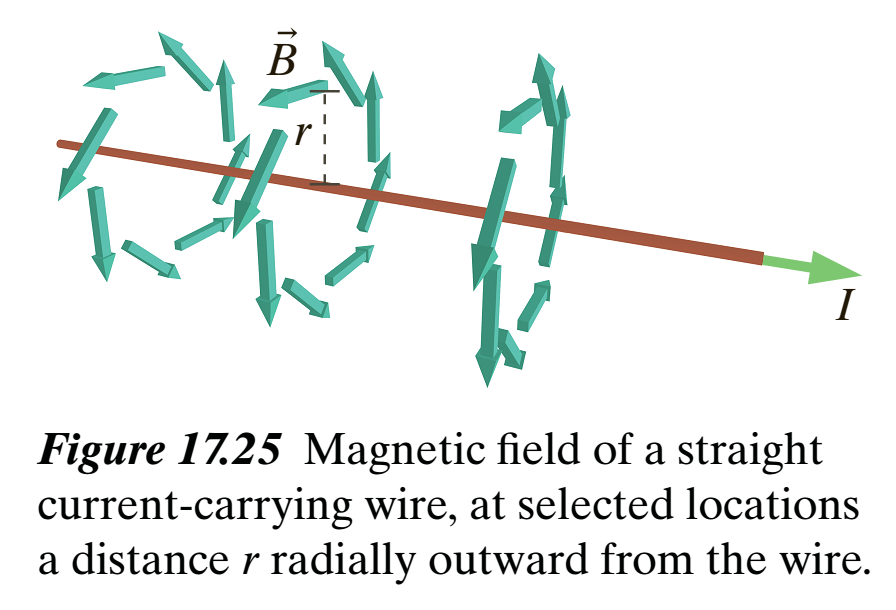
\includegraphics[height=3cm]{magneticField_wire_matterAndInteractions}
%\caption{text}
\end{Figure}

The magnetic field curls around the current-carrying wire (this direction is denoted $\hat{\theta}$ in cylindrical coordinates).  The magnitude of the magnetic field a distance $r$ from the wire is $|\vec{B}| = \frac{\mu_0 I}{2\pi r}$.

\subsection{Magnetic field due to a current-carrying loop}

\begin{Figure}
\centering
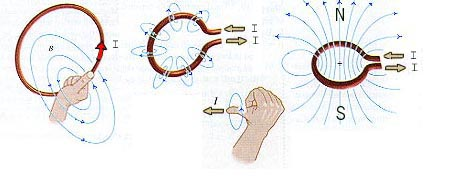
\includegraphics[height=3cm]{fieldofcircularloopfourviews}
%\caption{text}
\end{Figure}



The magnetic field of a loop of current is similar to the electric field of a dipole.

Along the loop axis, the magnetic field points along the axis.  The magnitude of the magnetic field a distance $x$ from the loop along the axis is $|\vec{B}|=\frac{\mu_0Ia^2}{2(x^2+a^2)^{3/2}}$ 

\section{Electric Field}
%Electric fields are relevant to circuits when working with capacitors (to calculate $\Delta V = -\int\vec{E}\cdot\vec{dl}$ one needs to know the electric field $\vec{E}$.  In addition, when considering the operation of circuits one needs to know the electric field to evaluate the forces experienced by the mobile electrons.
\subsection{Electric Field due to accelerating charges}
A \emph{changing} magnetic field is associated with a ``curly'' electric field.

\begin{Figure}
\centering
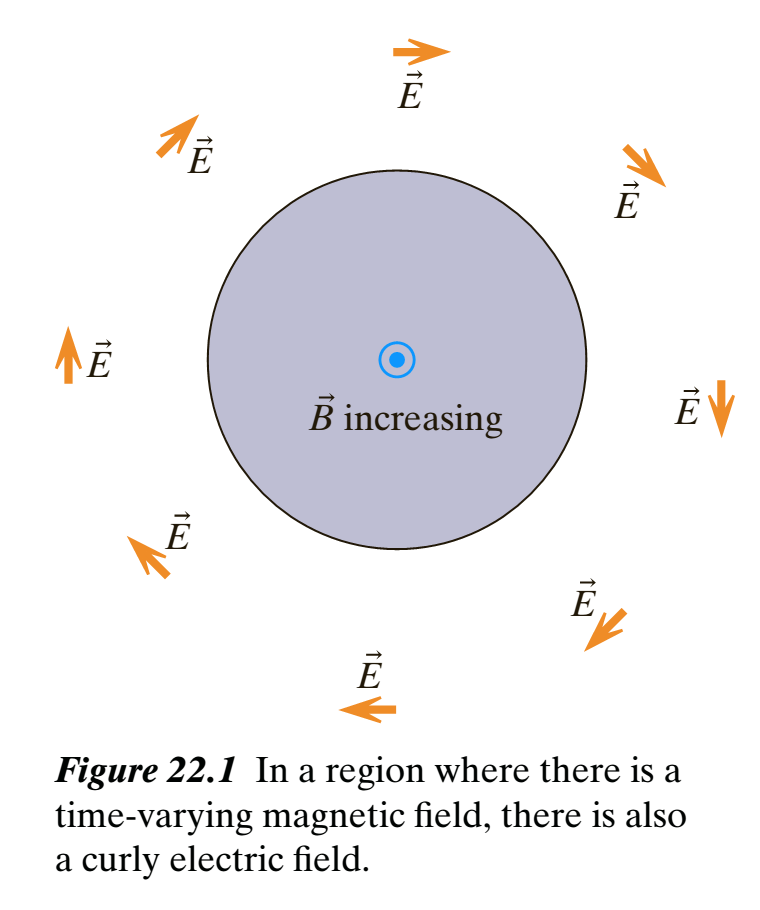
\includegraphics[height=3cm]{faraday1}
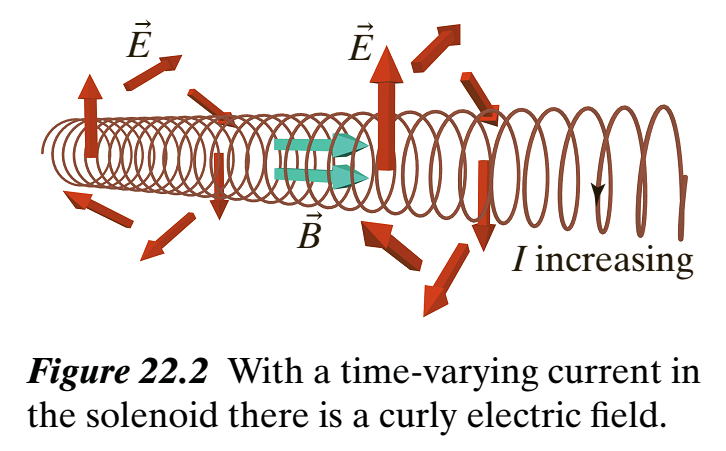
\includegraphics[height=3cm]{faraday2}
%\caption{text}
\end{Figure}

Faraday's law gives the magnitude of this electric field:
$\oint\vec{E}\cdot\vec{dl} = -\frac{d}{dt}\int\vec{B}\cdot\hat{n}\,dA$, or

$emf = \Delta V = -\frac{d}{dt} \phi_B$.

Notice that if the flux $\phi_B$ is constant (not changing), there is no associated electric field and therefore no potential.

To find the direction of the electric field, point your thumb in the direction of $-\Delta B$.  Your fingers then curl along $\vec{E}$.

\subsection{Electric Field due to a point-like Object}
The electric field due to a small, point-like object with net charge $Q$ is measured to be $\vec{E}=\frac{1}{4\pi\epsilon_0}\frac{Q}{r^2}\hat{r}$.

All electric fields can be derived from this, together with the principle of superposition: $\vec{E} = \vec{E_1} + \vec{E_2} + \vec{E_3} + ...$ and allows us to calculated the electric field of an arbitrary, fixed charge distribution.

\subsection{Electric Field due to a charged wire}
The magnitude of the electric field due to a wire with length L and net charge Q is approximately $\frac{1}{4\pi\epsilon_0}\frac{2Q/L}{r}$, where $r$ is the smallest possible distance to the wire.  This is a good approximation if the length of the wire $L$ is much larger than the distance from the wire $r$.  The direction of the electric field is radially outward from the wire if the charge is positive and radially toward the wire if the charge is negative.

\begin{Figure}
\centering
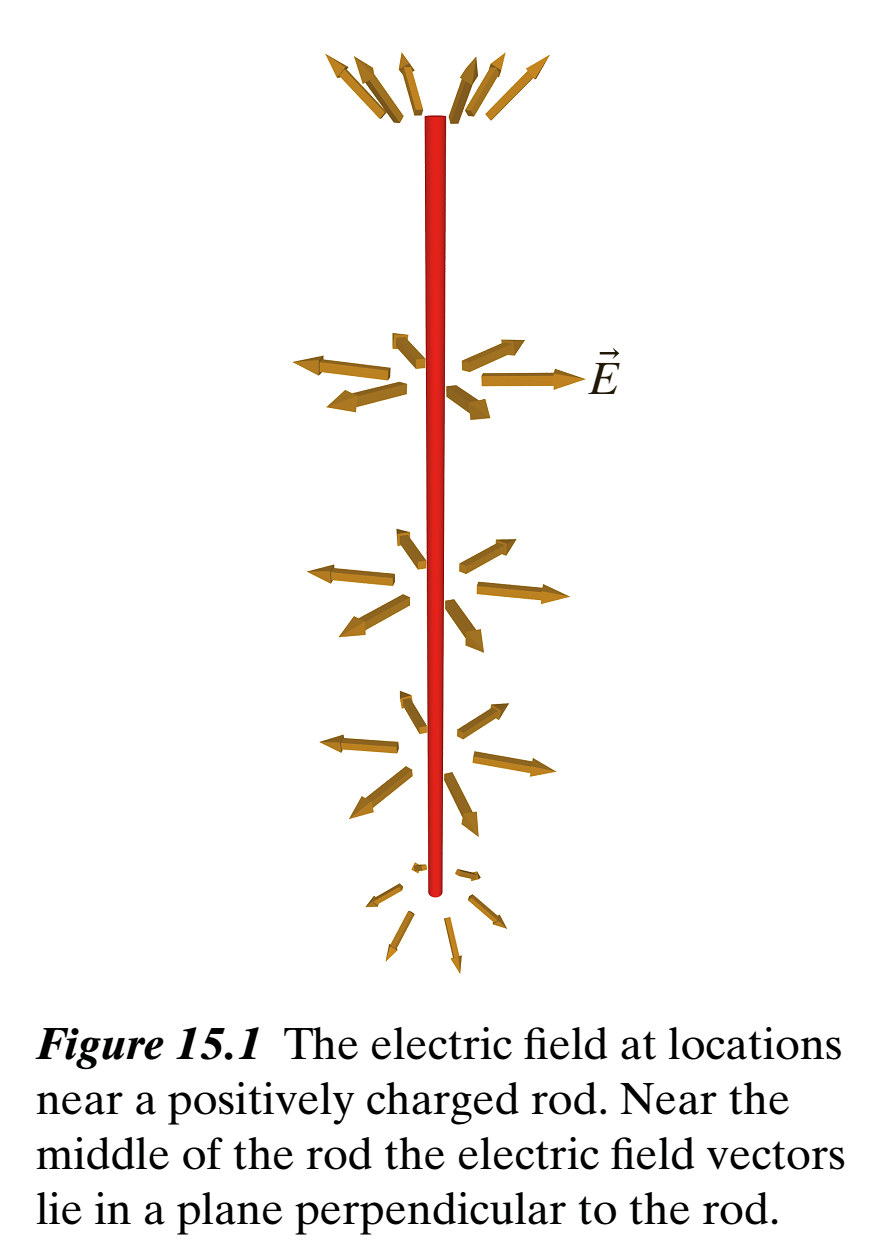
\includegraphics[height=5cm,angle=270]{Efield_wire_matterAndInteractions.PNG}
%\caption{text}
\end{Figure}	


\subsection{Electric Field due to a charged plane}
The magnitude of the electric field due to a large, charged plane is approximately $\frac{Q/A}{2\epsilon_0}$.  (Note that this does not depend on the distance from the plate.)  The direction of the electric field is away (perpendicular) from the plane if the plane is positively charged and towards (perpendicular) the plane if the plane is negatively charged.
\begin{Figure}
\centering
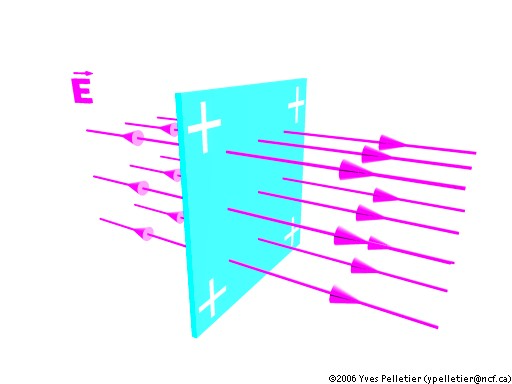
\includegraphics[height=3cm]{eField_plane}
%\caption{text}
\end{Figure}

\section{Electric Potential}
The change in electric potential $\Delta V$ is defined as $\Delta U / q$.  Note that the definition of $\Delta U$ above means that $\Delta V \equiv -\int\vec{E}\cdot\vec{dl}$.

%In some cases we talk about the electric potential at a point in space.  By convention, we mean $V_A = V_A - V_{\inf} = V_A - 0$.

%The electric potential at a point a distance $r$ from a point charge $Q$ is $V = \frac{1}{4\pi\epsilon_0}\frac{Q}{r}$.

\section{Inductance, LC Circuits}
Inductance $L$ measures how much a circuit element opposes changes in current, $|V| = L|\frac{dI}{dt}|$.

The inductance of a solenoid is $L = \frac{\mu_0 A N^2}{d}$, where $A$ is the cross-sectional area of the solenoid, $N$ is the number of turns of the wire creating the solenoid, and $d$ is the length of the solenoid.

In a circuit consisting of a solenoid and capacitor, charge will oscillate (!) with frequency $f = \frac{1}{2\pi\sqrt{LC}}$, where $f$ has units of cycles/time. 

\section{Vectors}
If point $S$ is located at $(x_1, y_1, z_1)$ and point $P$ is located at $(x_2, y_2, z_2)$ then the vector from point $S$ to point $P$ can be written: $\vec{r} = (x_2 - x_1)\hat{x} + (y_2 - y_1)\hat{y} + (z_2 - z_1)\hat{z}$.  The length of that vector is also called its magnitude and is denoted $|\vec{r}|$, where $|\vec{r}| = \sqrt{(x_2 - x_1)^2 + (y_2 - y_1)^2 + (z_2 - z_1)^2}$.  The magnitude of $\vec{r}$ is sometimes denoted simply by $r$.

\subsection{Unit Vectors}
A unit vector is a vector with magnitude one (``unity'') and is denoted with a hat: $\hat{r} = \vec{r}/|\vec{r}|$.

\subsection{Cross Product}
The cross product between two vectors results in a vector perpendicular to both those vectors.  If two vectors are parallel, their cross product is zero.

\begin{align*}
\vec{a}\times\vec{b} &= 
\begin{vmatrix}
\hat{x} & \hat{y} & \hat{z} \\
a_x & a_y & a_z \\
b_x & b_y & b_z
\end{vmatrix} \\
     &= \hat{x}(a_yb_z-a_zb_y) - \hat{y}(a_xb_z - a_zb_x) + \hat{z}(a_xb_y - a_yb_x)    \\           
&= |\vec{a}||\vec{b}|\sin{\theta}~\hat{a}\times\hat{b}
\end{align*}

Note that $\hat{x}\times\hat{y} = \hat{z}$.  Also note that the order of the vectors matters:  $\vec{a}\times\vec{b} = -\vec{b}\times\vec{a}$.

\subsection{Dot Product}
The dot product between two vectors results in a scaler and measures the ``overlap'' between two vectors.  If two vectors are perpendicular, their dot product is zero.  

\begin{align*}
\vec{a}\cdot\vec{b} &= a_x*b_x + a_y*b_y + a_z*b_z \\
                    &= |\vec{a}||\vec{b}|\cos{\theta}
\end{align*}
                  
Note that $\hat{x}\cdot\hat{x} = 1$ while $\hat{x}\cdot\hat{y} = 0$.

\begin{Figure}
\centering
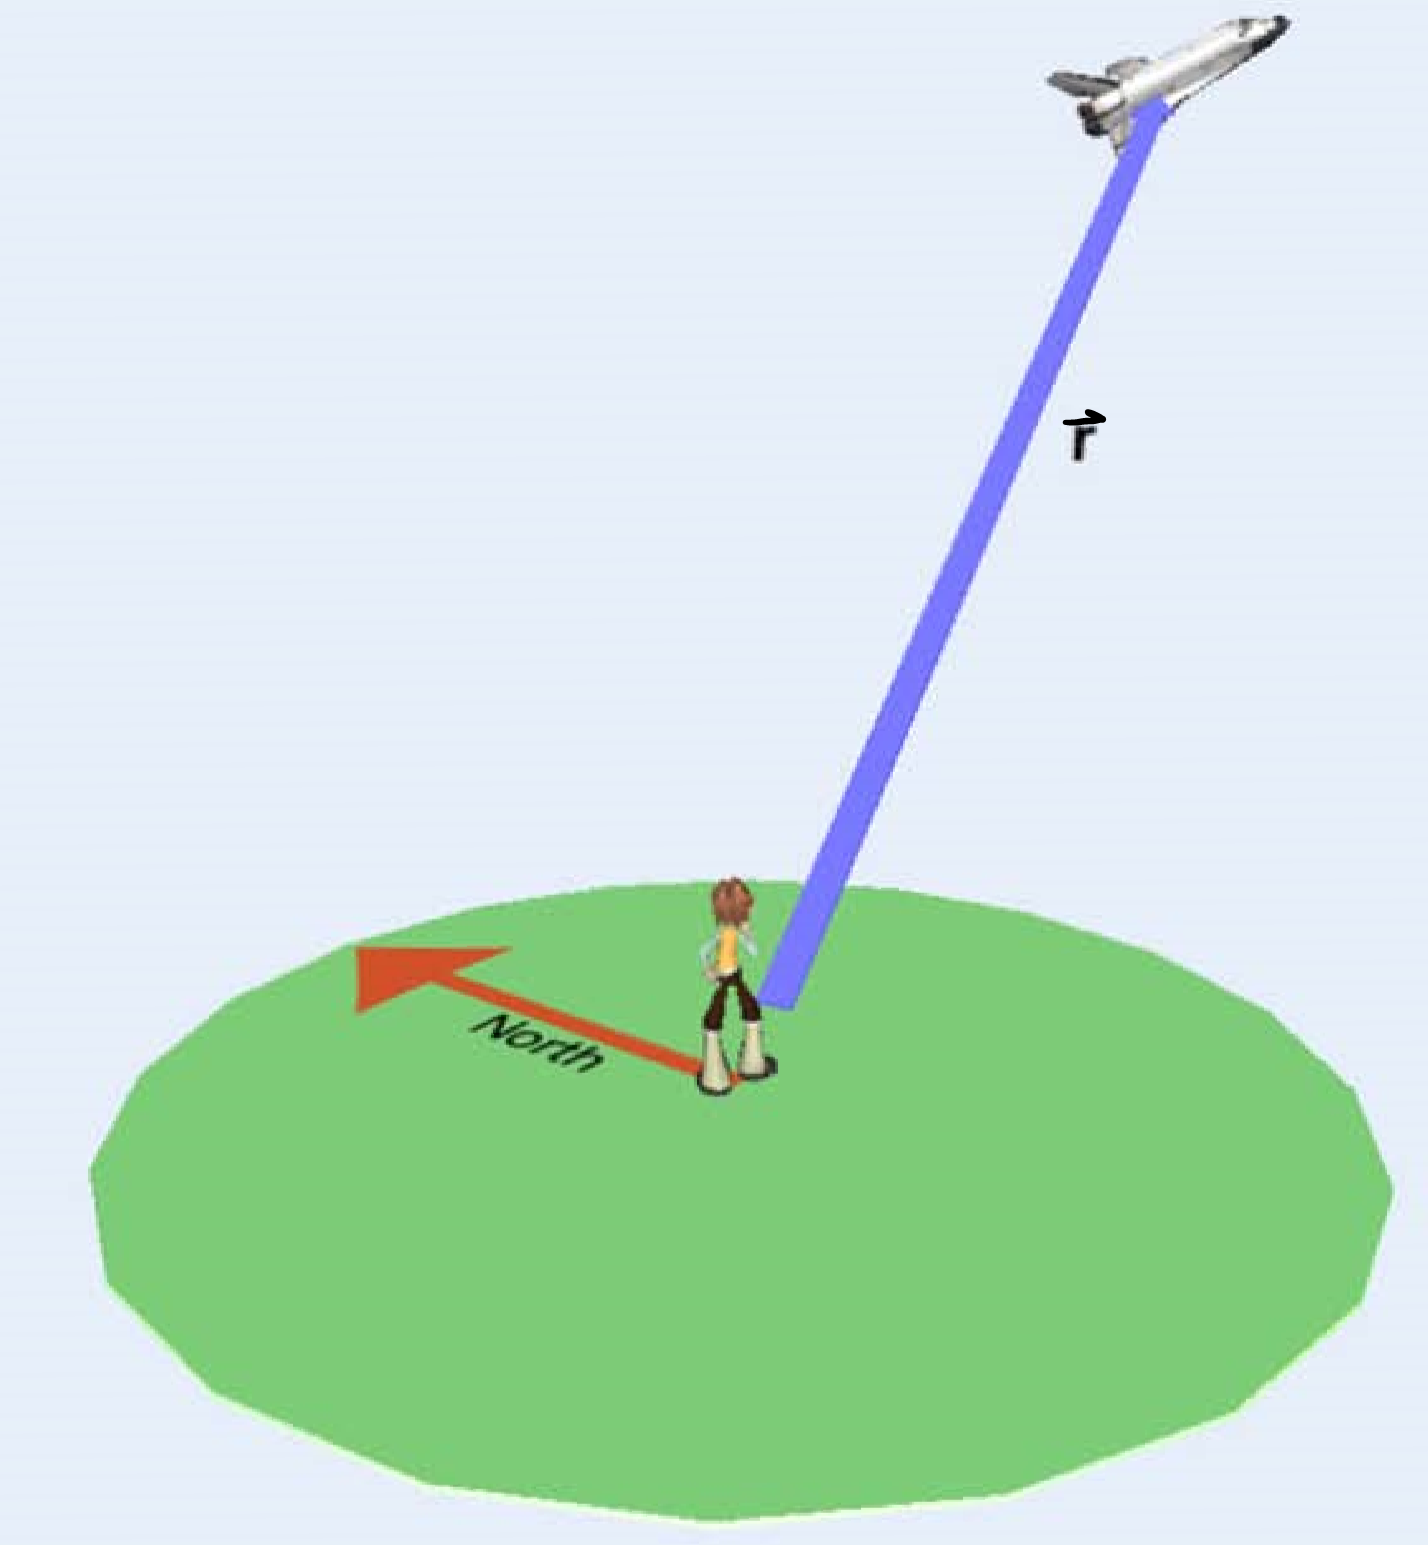
\includegraphics[width=0.9\textwidth]{r_vector.PNG}
%\caption{text}
\end{Figure}

\section{Batteries}
A battery is a chemical machine that provides a constant potential (voltage) across its terminals.  

\begin{Figure}
\centering
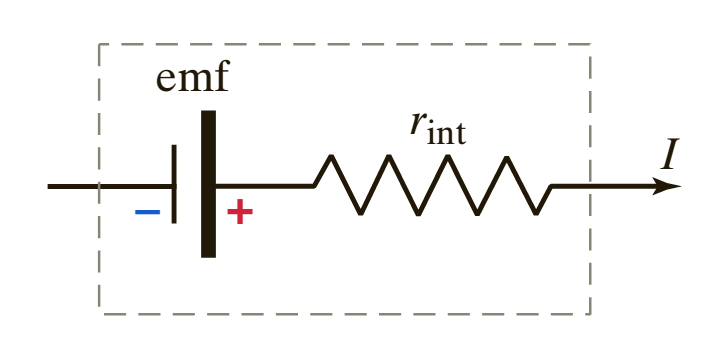
\includegraphics[height=2cm]{nonideal_batter_matterAndInteractions.PNG}
%\caption{text}
\end{Figure}	

\section{Conservation of Charge and Energy (Kirchoff's Laws)}
In any circuit loop, the total potential difference must be zero, or $\sum \Delta V = 0$

At any node in a circuit, the current flowing in must be the same as the current flowing out, or $i_1 = i_2 + i_3$.

\begin{Figure}
\centering
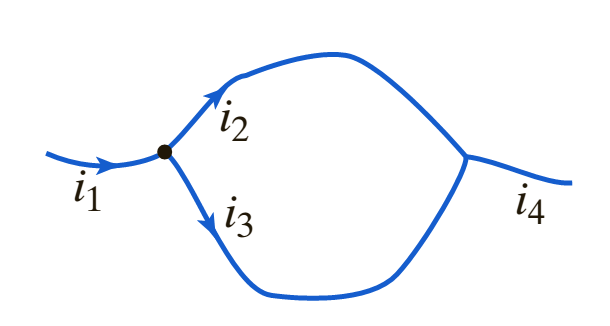
\includegraphics[height=3cm]{kirchoff_node_matterAndInteractions.PNG}
%\caption{text}
\end{Figure}

\section{Circuit Elements in Parallel and Series}
Resistors in series: $R = R_1 + R_2 + R_3 + ...$

Resistors in parallel: $\frac{1}{R} = \frac{1}{R_1} + \frac{1}{R_2} + ...$

Capacitors in series: $\frac{1}{C} = \frac{1}{C_1} + \frac{1}{C_2} + ...$

Capacitors in parallel: $C = C_1 + C_2 + C_3 + ...$

\section{Power dissipation in circuits}
Electrons flowing through resistive material warm up the material.

The power dissipated in a circuit can be written $P = IV = I^2R$.

\section{Charging and Discharging a Capacitor}
Capacitors store charge - and how fast they discharge is determined by both the resistance and capacitance of the circuit.
The charge on a discharging capacitor decays exponentially: $Q(t) = Q_0 e^{-t/RC}$.

\section{Constants}

$\frac{1}{4\pi\epsilon_0} = 9\times 10^9 N/Cm^2$ \newline
$\epsilon_0 = 8.85\times 10^{-12} {Cm^2/N}$ \newline
$\mu_0 = 4\pi\times 10^{-7} Tm/A$\newline
charge of an electron (denoted $-e$) = $-1.6\times 10^{-19} C$\newline
charge of a proton (denoted $e$) = $1.6\times 10^{-19} C$\newline
mass of an electron = $9.1\times 10^{-32} kg$ \newline
mass of a proton = $1.673\times 10^{-27} kg$ \newline
acceleration due to gravity (near the Earth's surface) = $9.8 N/kg = 9.8 m/s^2$ \newline
gravitational force constant $G$ = $6.67\times 10^{-11} Nm^2/kg$

% You can even have references
\rule{0.3\linewidth}{0.25pt}
\scriptsize
\bibliographystyle{abstract}
\bibliography{refFile}
\end{multicols}


\end{document}
